\apendice{Documentación técnica de programación}

\section{Introducción}
En esta sección se explicaran los conceptos necesarios para poder ponerse a trabajar con este proyecto:\\

Se tiene que descargar desde aquí: \\

\url{https://github.com/Guillecal/TFG-Herramienta_para_medir_la_eficiencia_de_codigo_python/tree/master/Prueba%20TFG\\}

\section{Estructura de directorios}

Los archivos necesarios están metidos en la carpeta Pruebas TFG, dentro de esta esta el archivo principal Vent.py que hace de controlador y vista, y este llama al interprete que  se encuentra dentro de la carpeta byterun. Dentro de esta nos interesa el archivo pyvm2.py que es donde se realizó el upgrade, ademas de ser la parte más importante del intérprete.\\

\section{Manual del programador}
Se empezará preparando el entorno de trabajo para trabajar con el proyecto:\\

\subsection{Python}
Para el desarrollo de la herramienta se utilizó la versión de Python 2.7.16, es recomendable descargar esta versión para evitar algún tipo de incoherencia.\\

Link de descarga: \url{https://github.com/Guillecal/TFG-Herramienta_para_medir_la_eficiencia_de_codigo_python/tree/master/Prueba%20TFG\\}

Seguido a esto es necesario instalar las bibliotecas utilizadas dentro del programa. Por ello es necesario comprobar si se tiene instalado primero el sistema de gestión pip, el cual es esencial para poder instalar las bibliotecas que se tengan.
Para este proyecto se utilizó la versión 19.1.1, pero en este caso la versión no debería afectar, hay que descargar el contenido que se encuentra en la siguiente dirección, guardar como get-pip.py:\\

Link Descarga: \url{https://bootstrap.pypa.io/get-pip.py}

Después de de esto en el símbolo de sistemas hay que ejecutar el comando: 
\begin{itemize}
	\item pip python get-pip.py
\end{itemize}

Cuando ya se tiene pip instalado ya solo sería meter los siguientes comandos por el símbolo de sistema:\\
\begin{itemize}
	\item pip install matplotlib
	\item pip install python-tk
\end{itemize}


\subsection{IDE}
Como entorno de desarrollo se puede utilizar el IDE de Python, pero para el desarrollo de la herramienta se ha utilizado Spyder. \\

Link descaga: \url{https://www.spyder-ide.org}\\

Una vez descargado e instalado este IDE ya viene listo para poder empezar a trabajar, pero en caso de que se requiera, se puden cambiar algunas configuraciones según el gusto de cada uno desde las pestañas Ver y Herramientas.\\

\begin{figure}[H]
\centering
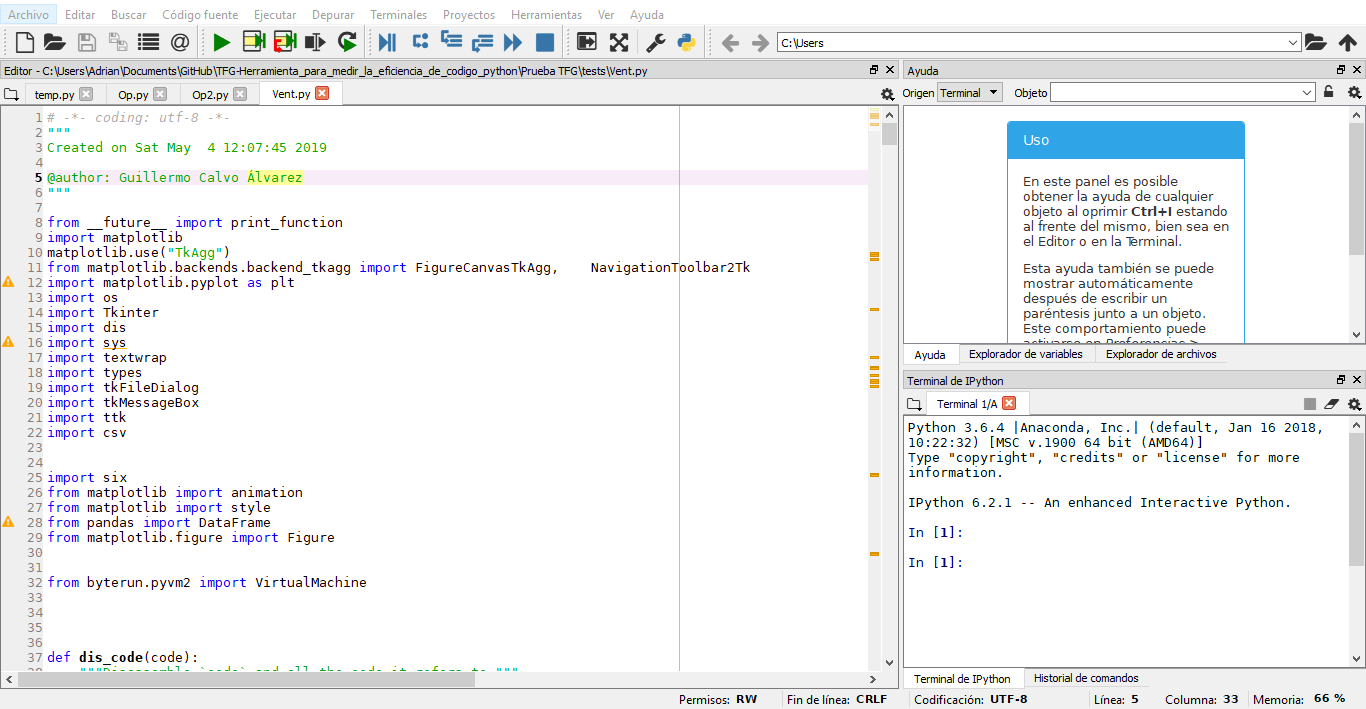
\includegraphics[width=11cm, height=7cm]{Spyder}
\caption{Así luce la ventana de Spyder}
\end{figure}

Esta es una recomendación, si se está acostumbrado utilizar otro tipo de IDE que sirva para el lenguaje Python no habría ningún problema.\\

\subsection{Github Desktop}

Esta es la herramienta utilizada para gestionar mejor el repositorio donde se encuentra el trabajo
Se puede descargas desde aquí: \\

Link: \url{https://desktop.github.com/}\\

Una vez descargado e instalado, la primera vez que lo ejecutamos, podemos clonar desde aquí el proyecto desde el repositorio

\section{Compilación, instalación y ejecución del proyecto}
No se puede compilar al ser Python el lenguaje del código, ya que este es un lenguaje interpretado. Tampoco es necesaria una instalación, por cual lo único que queda por hacer es ejecutar el código.
Hay dos maneras de hacer esto:\\

\begin{itemize}
	\item A través de la línea de comandos
	\item A través de un archivo ejecutable
\end{itemize}


\subsection{Linea de comandos}
Esta forma es muy sencilla. Simplemente hay que abrir el Símbolo de sistema(Línea de comandos) y navegar hasta el directorio donde se encuentra el archivo Vent.py, esto se puede hacer fácilmente con el comando CD para cambiar de directorio y dir para mostrar los que contiene el directorio actual.\\
Una vez encontrado el directorio simplemente hay que ejecutar el comando: Python Vent.py\\

\subsection{Archivo ejecutable}
Simplemente sería clicar en el archivo .exe que se encuentra dentro de la carpeta dist.\\

Pero para crear este archivo es necesario previamente haber configurado un fichero llamado setup.py que se tiene que encontrar en el mismo directorio que el archivo que se quiere hacer ejecutable, en nuestro caso es dentro de la carpeta prueba TFG. Setup.py se ha configurado de la siguiente manera: \\

\begin{figure}[H]
\centering
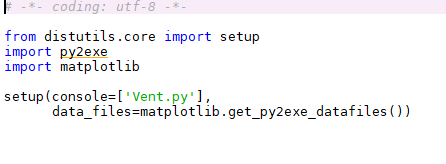
\includegraphics[width=8cm, height=5cm]{Setup}
\caption{Configuración del fichero setup.py}
\end{figure}

Una vez configurado hay que dirigirse al directorio donde se encuentran desde el símbolo de sistema y ejecutar el comando "setup.py py2exe". Con esto deberia generarse una carpeta llamada "dist" y dentro de este se encontrara el ejecutable\\

Como advertencia hay que comentar que podría ser necesario la descarga de un archivo .dll si no se tienen dentro de los archivos de python. 


\section{Pruebas del sistema}
Se han realizado dos vídeos, uno haciendo una prueba del análisis individual y otro haciendo el análisis múltiple. A parte también se comentan los contenidos de los archivos .csv\\